\chapter{Introduction}

\section{Motivations}
Aerial imagery is an important resource for applications that include urban planning and map-making \cite{5523977}. Ribbon-like features such as sidewalks, street networks, canals, or biking paths are especially important because they provide essential connections between sites to support transportation of people and materials. Any damage or obstacle appeared on these ribbon-like features may cause problems or hurt individual people. High-resolution aerial imagery has become a way to capture the appearance of these structures in order to look for changes such as new construction, degradation or damage, or obstructions. Geometrically, walking paths are thin features that can be described by a trajectory with varying thickness\cite{10.1007/11744078_9}. The scope of this thesis is automatic refinement of ribbon-like features: given an approximate trajectory and range of potential thicknesses, we automate the process of estimating the thicknesses and trajectory. One example of a downstream application would be an automatic method for precise localization and assessment of the quality of these pathways from geometric referenced imagery. Which could enable accurate walking instructions for people including those with disabilities that prevent them from moving around or seeing obstacles\cite{ZOU2012227}. 

\begin{figure}
    \centering
    \includegraphics[width=0.57\textwidth]{Figures/Goal.png}
    \caption[Objective Demonstration]{A demonstration on our approach. The first row shows the given input and the second row shows the output, with edges marked in red. We output the edges information as a .geojson file which allow us to edit and change with the given input file.}
    \label{fig:goal}
\end{figure}


Public domain or crowd-sourced repositories of spatial data such as \ac{OSM} \cite{OpenStreetMap} represent a very complete and frequently updated source of information which includes street vector data, and to a much lesser extent, the locations of foot-ways. However, the data is acquired from a variety of sources that may not be registered with enough precision to accurately place thin features such as walking paths. For thin structures such as sidewalks that are visible in \ac{VHR} imagery, even small discrepancies between the digitized pathways and the imagery can be distracting when used to visualize an overland map. As new \ac{VHR} aerial imagery becomes available thin features such as walking paths are discernible with higher precision, but ortho-rectification processes may not precisely align the imagery with previously digitized features. In addition, poorly registered walking paths could confound any algorithm that might hope to automatically locate features on the path including obstacles, damage, overgrowth, or stairways that could impact the walk-ability. In addition, several authors\cite{femiani2009interval, femiani2007road} have worked on segmenting streets and sidewalks or other linear features directly from aerial imagery; however sidewalks are much thinner than streets and are often partially occluded. More importantly, these methods are mainly concerned with the connectivity of the extracted pathways and not with identifying the precise boundaries. Figure \ref{fig:goal} shows the input and desired output with our approach, we marked the boundaries as red. Figure \ref{fig:fw_ov} demonstrate the step by step detail diagram for our approach, from the input map (a), along with the initial trajectory(b), we can generate the ribbon-image with the given mid-curve(c). We generate the initial estimation for each pixels(d) with \ac{GMM} along the ribbon-image, then apply our approach with \ac{DP} solution(e). Our approach can be used to refine or recover the thickness of street networks or other networks of ribbon-like features. Several automatic approaches model segmentation as a \ac{CRF} in order to ensure that the resulting output configurations are plausible \cite{ActiveContou09, Rother2004-ou, Achanta:149300}.

\begin{figure}[H]
    \centering
    \includegraphics[width=0.75\textwidth]{Figures/diagram6.png}
    \caption[Framework Overview 1]{Our 6 step approach adopted to predict precise boundaries for ribbon-like features. (a) Input Map, (b) Initial Trajectory, (c) Ribbon Image Generation, (d) Density Estimation for Pixels, (e) Apply \ac{DP} Solution, (f) Reshape Sidewalk.}
    \label{fig:fw_ov}
\end{figure}

\section{Challenges}

\begin{figure}[H]
    \centering
    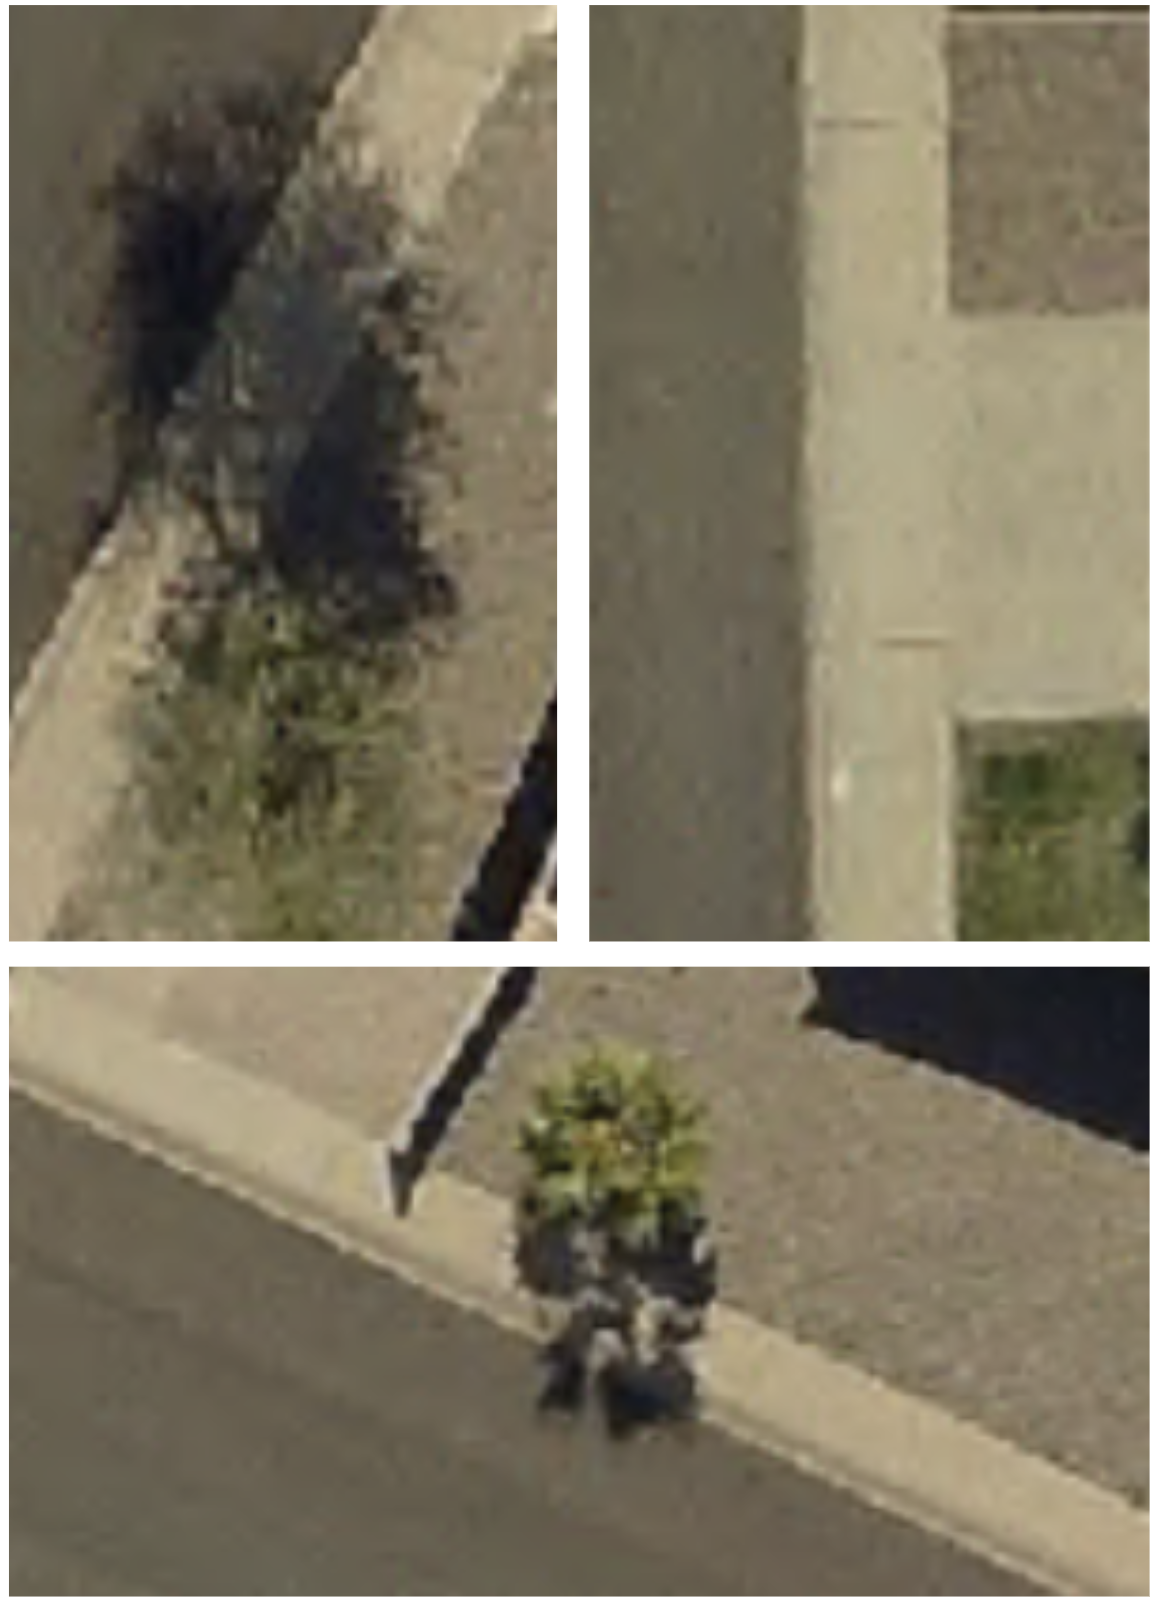
\includegraphics[width=0.8\textwidth]{Figures/challenge.png}
    \caption[Challenges Demonstration]{A detail demonstrations on challenges that we are facing in our approach. From left to right, top to bottom, it shows that sidewalk are under the shadow, camouflage with adjacent materials and blocked by obstacles.}
    \label{fig:challenge_demo}
\end{figure}

As shown in figure \ref{fig:challenge_demo}, the main challenge addressed by our approach is to predict precise boundaries for ribbon-like walking paths when they are:

\begin{itemize}
    \item blocked by obstacles,
    \item under the shadow of trees, cars, buildings,
    \item camouflage with adjacent materials (e.g. driveways, gutters),
    \item partially damaged so texture varies along the sidewalk.
\end{itemize}

Under the circumstances, most feature segmenting tools will not able to locate accurate boundaries, their results may recognize the non-sidewalk pixels (FP) as the sidewalk or the other way around (FN). 

\section{Contributions}

The aim of this work is to precisely align and determine the width of a coarsely registered ribbon-like feature to match its appearance in a \ac{VHR} image. The input is a \ac{VHR} georeferenced and orthorectified image along with a set of linear features that are close to, but perhaps not precisely aligned with the center of a ribbon-like feature. In particular, we expect that the ribbon will be made of a material with a somewhat uniform appearance (e.g. asphalt, gravel, or concrete) but that its appearance will be affected by shadows and interrupted by occlusions from vegetation, pedestrians, or vehicles such as bicycles. Our aim is to determine a more precise mid-line and an estimate for the width of the ribbon-like feature, which can very slowly along its trajectory. The solution proposed in this paper does not rely on prior knowledge of the material on or around the ribbon, but instead, it estimates material appearance as it refines the placement of an initial estimate for the ribbon's mid-line.
	
	Our contributions are as follows:
	\begin{itemize}
		\item A novel \ac{DP} approach is proposed for aligning ribbon-like features to orthoimaagery.
		\item We do not require large training sets; a few parameters to control the smoothness of the resulting ribbon along with a coarse initial estimate of the trajectory are all that is needed.
		\item Unlike methods that aim to recover the trajectories only, in our approach a likely thickness is directly identified so that more plausible trajectories and boundaries can be identified.
		\item An application to the problem of registering sidewalks to aerial photographs is demonstrated, allowing \ac{GIS} data sets to be improved as high-resolution ortho imagery becomes available. 
	\end{itemize}